\documentclass[a4paper]{article}
\usepackage{graphicx}
\usepackage[utf8]{inputenc}
\usepackage[english, serbian]{babel}

\title{UseCase: Promena korisničkih podataka}
\date{12.11.2018.}

\begin{document}

\maketitle

\begin{itemize}
    \item Akter: Administrator
    \item Kratak opis: Korisnik želi da promeni neke od ličnih podataka drugih korinika
    \item Osnovni tok događaja:
        \begin{enumerate}
            \item Administratoru se prikazuje panel u kojem se nalazi spisak korisnika kojima može menjati lične informacije.
            \item Administrator bira željenog korisnika.
            \item Administratoru se prikazuje formular na kome može menjati lične podatke korisnika (sve osim email-a).
            \item Nakon uspešne promene podataka sistem obaveštava administratora o uspešnoj akciji.
        \end{enumerate}
    \item Alternativni tok događaja:
        \begin{enumerate}
            \item Neko od obaveznih polja nije popunjeno ili neko od polja ne odgovara formatu koji je za to polje zadat regularnim izrazom
                \begin{enumerate}
                    \item Nakon 2. koraka sistem ispisuje poruku o grešci i obaveštava administratora da podaci nisu uspešno izmenjeni.
                    \item Administrator se vraća na korak 3 glavnog toka.
                \end{enumerate}
        \end{enumerate}
\end{itemize}

\begin{figure}
    \centering
    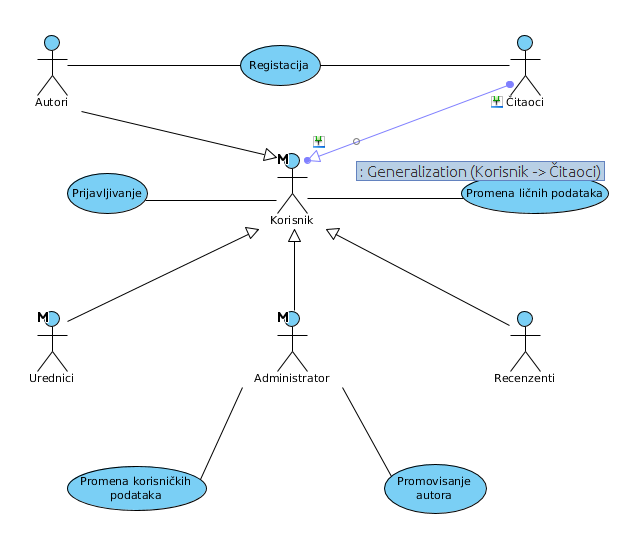
\includegraphics[width=\linewidth]{usecasePrijavljivanje.png}
    \caption{UseCase screenshot}
    \label{fig:my_label}
\end{figure}


\end{document}
